%% This is an example first chapter.  You should put chapter/appendix that you
%% write into a separate file, and add a line \include{yourfilename} to
%% main.tex, where `yourfilename.tex' is the name of the chapter/appendix file.
%% You can process specific files by typing their names in at the 
%% \files=
%% prompt when you run the file main.tex through LaTeX.

\chapter{Evaluación Experimental}

Inicialmente para comprobar este método se presentó a los usuarios una descripción de un anuncio de auto creado por Chevrolet y una descripción de una hamburguesa creada por Carl's Jr que eran comparados con dos anuncios creados por nuestro método, una descripción de un anuncio de un auto se comparaba con el anuncio de Chevrolet y una descripción de un anuncio de una hamburguesa se comparaba con el anuncio de Carl's Jr. Los resultados obtenidos fueron muy satisfactorios superando en preferencia del usuario el anuncio optimizado al anuncio creado por el experto. Con estos resultados pudimos darnos una idea del potencial de este método y continuar con las siguientes pruebas.


\section{El Método de Evaluación}

En nuestro método de evaluación la medición de la eficiencia de un anuncio de texto se realizó mediante la comparación de una versión que resultó de la evolución de los textos, contra una versión construida por un experto. Para los experimentos, una persona especializada en un área relacionada con el marketing es considerado un experto.
 
Para la primera parte del experimento, se le podio a un grupo de 30 personas, elegidas al azar, que eligiera la versión que ellos pensaban que podría persuadirlos con mayor facilidad. El texto con mayoría de votos se consideraba como el que más persuadía a una persona a comprar el producto anunciado. Aunque esta prueba podría presentar defectos, dado que la mejor estrategia para medir la efectividad de un anuncio de texto sería ponerlo en la práctica real, la prueba puede producir una idea aproximada de los resultados reales. 

Esta parte del experimento se repite con cinco versiones diferentes de diferentes expertos, contra el mismo texto evolucionado. 

La prueba de reconocimiento consiste en mostrar a un grupo de 30 personas el sitio web ficticio, donde se presenta un trailer de una película  durante 30 segundos. Por encima de este video, se muestra el texto del anuncio. Al terminar el video, el sitio web se oculto del participante, y se le pregunta a los participantes si vieron algún anuncio mientras miraban el video. Si los participantes vieron el anuncio, esto significa que reconocieron el anuncio. Al final, el número de personas que reconocieron el anuncio de texto se divide entre el total de participantes en esa prueba, lo que representa el porcentaje de reconocimiento para el anuncio dado. 

La prueba de memoria se realiza después de la prueba de reconocimiento. Al mismo grupo de personas que participaron en la prueba de reconocimiento, y que reconocieron con éxito el anuncio, se le pregunta si recuerdan de que trataba el anuncio. Al igual que en la prueba de reconocimiento, el número de personas que recordaron el tema del texto se divide entre el número total de participantes, lo que representa el porcentaje de memoria para el anuncio dado. 

El sitio web puede apreciarse en la Figura \ref{experimento}. El video se puede ver a la derecha, y el anuncio de texto en su parte superior, rodeado con un borde azul.

\begin{figure}[htp]
  \centerline{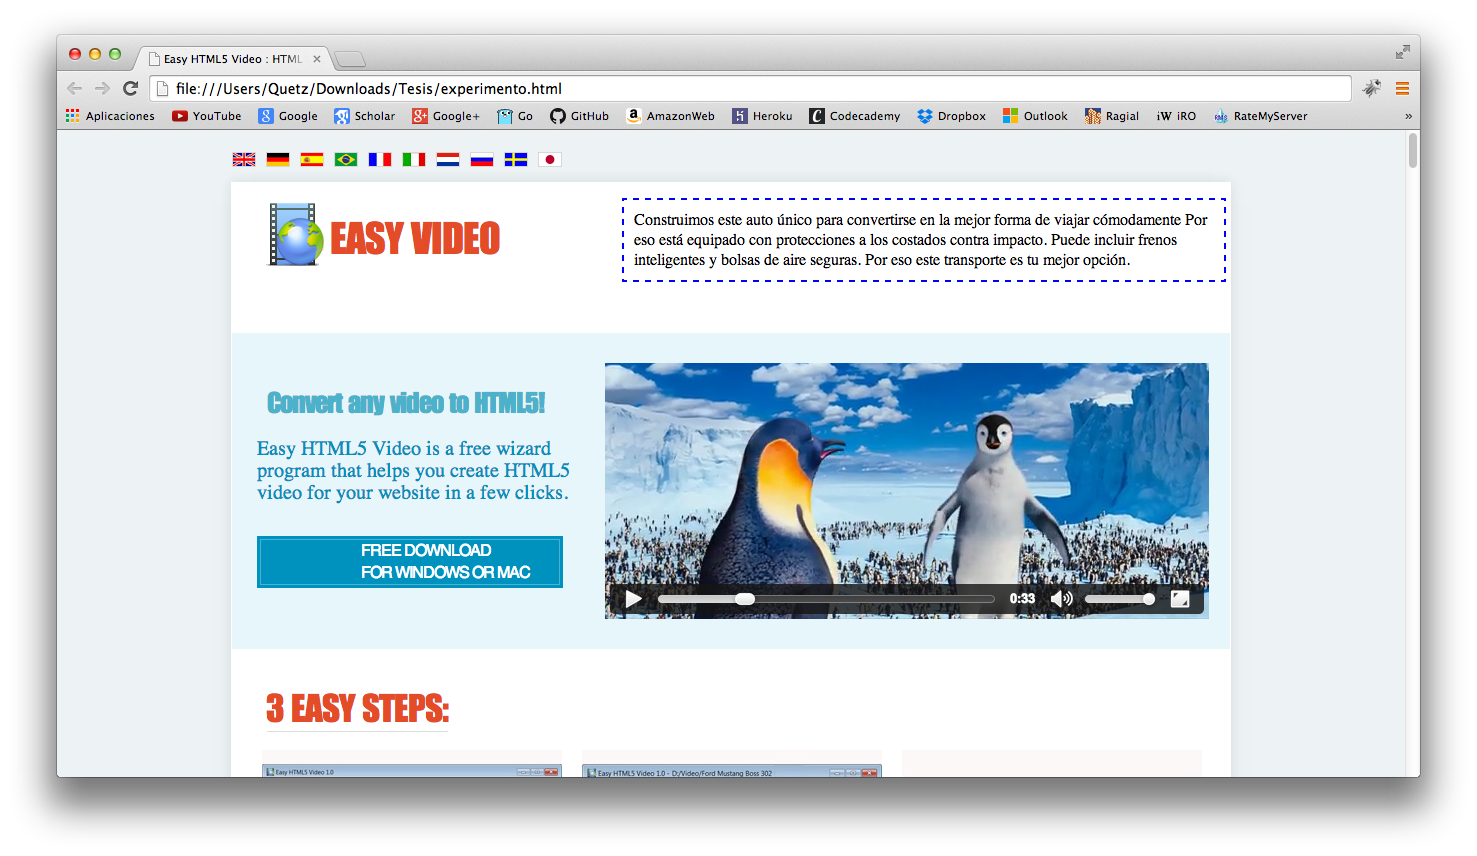
\includegraphics[width=7in]{experimento.png}} 
  \caption{Prueba de Reconocimiento y Memoria } 
\label{experimento}
\end{figure}

\section{Resultados}

La Tabla \ref{hamburgusa} presenta los resultados de los experimentos llevados a cabo utilizando el texto publicitario de la hamburguesa, mientras que la Tabla \ref{auto} se presentan los resultados del texto publicitario del automóvil.
Los porcentajes que se muestran en las tablas representan las calificaciones dadas por los participantes para cada versión de texto del anuncio. Por ejemplo,  el 60\%, significa que 60 personas de las 150 personas que participaron en el experimento, reconocía o recordaba el texto con éxito. En la prueba de la persuasión, los resultados son complementarios, lo que significa que, por ejemplo, el 56\% de los participantes prefirió la versión evolucionada del texto de la hamburguesa, mientras que el 44\% de los participantes prefirieron la versión del experto. 
Como se mencionó en la Sección 7.1, 30 personas participaron en cada parte del experimento. Se necesitaban 150 personas diferentes para cada prueba, ya que cada parte se realizó cinco veces (el texto evolucionado compitió contra cinco opciones diferentes expertos).

\begin{table}
\begin{center}
\begin{tabular}{|r|c|c|}
Tipo de Prueba & Promedio General (Evolucionado) & Promedio General (Experto) \\\hline \hline

Reconocimiento & 40\% & 46\% \\
Memoria & 27.3\% & 22\% \\
Persuasion & 56\% & 44\% \\

\end{tabular}
\end{center}
\caption{Resultados del experimento con el anuncio de la hamburguesa}
\label{hamburgusa}
\end{table}



\begin{table}
\begin{center}
\begin{tabular}{|r|c|c|}
Tipo de Prueba & Promedio General (Evolucionado) & Promedio General (Experto) \\\hline \hline

Reconocimiento & 65.3\% & 54.6\% \\
Memoria & 32.6\% & 24\% \\
Persuasion & 54\% & 46\% \\
\end{tabular}
\end{center}
\caption{Resultados del experimento con el anuncio de el automovil}
\label{auto}
\end{table}
